\documentclass[twoside,10pt]{article}
%=================================================
% Basics
%=================================================
\usepackage{fixltx2e} % Makes \( \) equation style robust, among other
                      % things. Must be the first package.


% Makes ligatured fonts searchable and copyable in pdf readers
\usepackage{cmap} % Load before fontenc 

% Always include these font encodings in your document 
% unless you have a very good reason.
\usepackage[T1]{fontenc}
\usepackage[utf8]{inputenc}

\usepackage{verbatim}

%=============
% Fonts
%=============

\usepackage{lmodern} % Improved version of computer modern
\usepackage[scale=0.88]{tgheros} % Helvetica clone for sans serif font


\newcommand\hmmax{2} % Default is 3.
\newcommand\bmmax{2} % Default is 4.

\usepackage{bm} % boldmath must be called after the package
\providecommand{\mathbold}[1]{\bm{#1}}

%=============
% AMS Packages and fonts
%=============
\usepackage{amsmath,amsbsy,amsgen,amscd,amsthm,amsfonts,amssymb} 

%=============
% Margins and paper size
%=============
\usepackage[centering,top=1.5in,bottom=1.2in,left=1.4in,right=1.4in]{geometry}
\usepackage{parskip}


%=============
% Section headings
%=============
\usepackage[sf,bf,compact]{titlesec}

%=============
% Tables and lists
%=============
\usepackage{booktabs,longtable,tabu} % Nice tables
\setlength{\tabulinesep}{1mm}
\usepackage[font=small,margin=10pt,labelfont={sf,bf},labelsep={space}]{caption}

%=============
% Code output
%=============
% \usepackage{listings}
% \usepackage{minted}




\usepackage{enumitem}
\setitemize{itemsep=0pt} 
\setenumerate{itemsep=0pt}
\setlist{labelindent=\parindent,%  % Recommended by enumitem package
  font=\sffamily}


%=============
% Hyperlink colors
%=============
\usepackage[usenames,dvipsnames]{xcolor}
\definecolor{steelblue}{HTML}{A1BDC7}
\definecolor{orange}{HTML}{D98C21}
\definecolor{silver}{HTML}{B0ABA8}
\definecolor{rust}{HTML}{B8420F}
\definecolor{seagreen}{HTML}{2E6B69}
\definecolor{joshua}{HTML}{FBDC7F}
\definecolor{darksky}{HTML}{154c79}

\colorlet{steelblue}{silver!30!white}
\colorlet{darkorange}{orange!85!black}
\colorlet{darksilver}{silver!85!black}
\colorlet{darksteelblue}{steelblue!85!black}
\colorlet{darkrust}{rust!85!black}
\colorlet{darkseagreen}{seagreen!85!black}

\usepackage{url}
\usepackage[colorlinks=true]{hyperref}
\hypersetup{linkcolor=darkrust}    
\hypersetup{citecolor=darkseagreen}      
\hypersetup{urlcolor=darksilver}     

%=============
% Microtype
%=============
\usepackage[final]{microtype} 

%=====================
% Header
%=====================
% \usepackage{fancyhdr}
% \usepackage{nopageno} % Gets rid of page number at the bottom
% \fancyhf{} % Clear header style
% \renewcommand{\headrulewidth}{0.5pt} % remove the header rule
% \pagestyle{fancy}
% \fancyhead[LE,RO]{\textsf{\small \thepage}}
% 
% \setlength{\headheight}{14pt}
%=====================
% Fix delimiters
%=====================

% Fixes \left and \right spacing issues. See discussion at
% http://tex.stackexchange.com/questions/2607/spacing-around-left-and-right
\let\originalleft\left
\let\originalright\right
\renewcommand{\left}{\mathopen{}\mathclose\bgroup\originalleft}
\renewcommand{\right}{\aftergroup\egroup\originalright}

%=================================================
% Math macros
%=================================================

%=============
% Generalities
%=============
\usepackage{mathtools}
\mathtoolsset{centercolon}  % Makes := typeset correctly for definitions

%%% Equation numbering
%\numberwithin{equation}{section} 

%%% Annotations
\newcommand{\notate}[1]{\textcolor{red}{\textbf{[#1]}}}

%==============
% Symbols
%==============
\let\oldphi\phi
\let\oldeps\epsilon

\renewcommand{\phi}{\varphi}
\renewcommand{\epsilon}{\varepsilon}
\newcommand{\eps}{\varepsilon}

%==============
% Constants
%==============

% Set constants upright
\newcommand{\cnst}[1]{\mathrm{#1}}  
\newcommand{\econst}{\mathrm{e}}

\newcommand{\zerovct}{\vct{0}} % Zero vector
\newcommand{\Id}{\mathbf{I}} % Identity matrix
\newcommand{\onemtx}{\bm{1}}
\newcommand{\zeromtx}{\bm{0}}

%==============
% Sets
%==============
\providecommand{\mathbbm}{\mathbb} % In case we don't load bbm

% Reals, complex, naturals
\newcommand{\R}{\mathbbm{R}}
\newcommand{\C}{\mathbbm{C}}
\newcommand{\K}{\mathbbm{K}}
\newcommand{\N}{\mathbbm{N}}

%==============
% Probability
%==============
\newcommand{\Prob}{\operatorname{\mathbbm{P}}}
\newcommand{\Expect}{\operatorname{\mathbb{E}}}

%==============
% Vectors and matrices 
%==============
\newcommand{\vct}[1]{\mathbold{#1}}
\newcommand{\mtx}[1]{\mathbold{#1}}

\newcommand{\mrange}{\operatorname{range}}
\newcommand{\mnull}{\operatorname{null}}



\newcommand{\Z}{\mathbbm{Z}}

\begin{document}

\title{CSE 6643 Homework 4}
\author{Karl Hiner}
\date{}
\maketitle

\section{Schur Complements I [25 pts]}
Consider the matrix 
\begin{equation}
  \mtx{M}
  \coloneqq
  \begin{pmatrix}
    \mtx{A} & \mtx{B}\\
    \mtx{C} & \mtx{D}
  \end{pmatrix}, 
\end{equation}
where $\mtx{A} \in \K^{m \times m}$ and $\mtx{D} \in \K^{n \times n}$ are square matrices.
The matrix $\mtx{M}/\mtx{A} \coloneqq \mtx{D} - \mtx{C} \mtx{A}^{-1} \mtx{B}$ is called the Schur complement of $\mtx{A}$ in $\mtx{M}$.    

\subsection*{(a) [5 pts]} 
  Relate the Schur complement $\mtx{M} / \mtx{A}$ to the block LU factorization of $\mtx{M}$.

  \quad The block LU factorization of $\mtx{M}$ is given by 
  \begin{equation*}
    \mtx{M} = 
    \begin{pmatrix}
      \mtx{I} & \mtx{0} \\
      \mtx{C} \mtx{A}^{-1} & \mtx{I}
    \end{pmatrix}
    \begin{pmatrix}
      \mtx{A} & \mtx{0} \\
      \mtx{0} & \mtx{M} / \mtx{A}
    \end{pmatrix}
    \begin{pmatrix}
      \mtx{I} & \mtx{A}^{-1} \mtx{B} \\
      \mtx{0} & \mtx{I}
    \end{pmatrix}.
  \end{equation*}
  \quad We can verify this by multiplying the terms and verifying we end up with $\mtx{M}$:
  \begin{align*}
    &\begin{pmatrix}
      \mtx{I} & \mtx{0} \\
      \mtx{C} \mtx{A}^{-1} & \mtx{I}
    \end{pmatrix}
    \begin{pmatrix}
      \mtx{A} & \mtx{0} \\
      \mtx{0} &\mtx{M} / \mtx{A}
    \end{pmatrix}
    \begin{pmatrix}
      \mtx{I} & \mtx{A}^{-1} \mtx{B} \\
      \mtx{0} & \mtx{I}
    \end{pmatrix}\\
    &= 
    \begin{pmatrix}
      \mtx{I} & \mtx{0} \\
      \mtx{C} \mtx{A}^{-1} & \mtx{I}
    \end{pmatrix}
    \begin{pmatrix}
      \mtx{A} & \mtx{A} \mtx{A}^{-1} \mtx{B} \\
      \mtx{0} & \mtx{M} / \mtx{A}
    \end{pmatrix}\\
    &= 
    \begin{pmatrix}
      \mtx{I} & \mtx{0} \\
      \mtx{C} \mtx{A}^{-1} & \mtx{I}
    \end{pmatrix}
    \begin{pmatrix}
      \mtx{A} & \mtx{B} \\
      \mtx{0} & \mtx{M} / \mtx{A}
    \end{pmatrix}\\
    &=
    \begin{pmatrix}
      \mtx{A} & \mtx{B}\\
      \mtx{C}\mtx{A}^{-1}\mtx{A} & \mtx{C}\mtx{A}^{-1}\mtx{B} + \mtx{M} / \mtx{A}
    \end{pmatrix}\\
    &=
    \begin{pmatrix}
      \mtx{A} & \mtx{B}\\
      \mtx{C} & \mtx{C}\mtx{A}^{-1}\mtx{B} + \mtx{D} - \mtx{C} \mtx{A}^{-1} \mtx{B}
    \end{pmatrix}\\
    &=
    \begin{pmatrix}
      \mtx{A} & \mtx{B}\\
      \mtx{C} & \mtx{D}
    \end{pmatrix} = \mtx{M}
  \end{align*}

\subsection*{(b) [5 pts]} 
  Show that the determinant of $\mtx{M}$ is given by $\det\left(\mtx{A}\right) \det\left(\mtx{M} / \mtx{A}\right)$.

  \quad Expressing $\mtx{M}$ as its block LU factorization:
\begin{align*}
  \mtx{M} &= 
  \begin{pmatrix}
    \mtx{I} & \mtx{0} \\
    \mtx{C} \mtx{A}^{-1} & \mtx{I}
  \end{pmatrix}
  \begin{pmatrix}
    \mtx{A} & \mtx{0} \\
    \mtx{0} & \mtx{M} / \mtx{A}
  \end{pmatrix}
  \begin{pmatrix}
    \mtx{I} & \mtx{A}^{-1} \mtx{B} \\
    \mtx{0} & \mtx{I}
  \end{pmatrix}\\
  \det(\mtx{M}) &= 
  \det\left(\begin{pmatrix}
    \mtx{I} & \mtx{0} \\
    \mtx{C} \mtx{A}^{-1} & \mtx{I}
  \end{pmatrix}
  \begin{pmatrix}
    \mtx{A} & \mtx{0} \\
    \mtx{0} & \mtx{M} / \mtx{A}
  \end{pmatrix}
  \begin{pmatrix}
    \mtx{I} & \mtx{A}^{-1} \mtx{B} \\
    \mtx{0} & \mtx{I}
  \end{pmatrix}\right)\\
  &= \det\left(\begin{pmatrix}
    \mtx{I} & \mtx{0} \\
    \mtx{C} \mtx{A}^{-1} & \mtx{I}
  \end{pmatrix}\right)
  \det\left(\begin{pmatrix}
    \mtx{A} & \mtx{0} \\
    \mtx{0} & \mtx{M} / \mtx{A}
  \end{pmatrix}\right)
  \det\left(\begin{pmatrix}
    \mtx{I} & \mtx{A}^{-1} \mtx{B} \\
    \mtx{0} & \mtx{I}
  \end{pmatrix}\right)\\
  &= 1 \cdot 
  \det\left(\begin{pmatrix}
    \mtx{A} & \mtx{0} \\
    \mtx{0} & \mtx{M} / \mtx{A}
  \end{pmatrix}\right)
  \cdot 1\\
  &= 
  \det\left(\mtx{A}\right)\det\left(\mtx{M} / \mtx{A}\right)\\
\end{align*}

\subsection*{(c) [7.5 pts]}
  Let $\mtx{M} = \mtx{L} \mtx{U}$ be the LU factorization of $\mtx{M}$. 
  Split its factors into block matrices 
  \begin{equation} 
    \mtx{L} = 
    \begin{pmatrix}
      \mtx{L}_{1, 1} & \mtx{0} \\
      \mtx{L}_{2, 1} & \mtx{L}_{2, 2}
    \end{pmatrix},
    \quad 
    \mtx{U} = 
    \begin{pmatrix}
      \mtx{U}_{1, 1} & \mtx{U}_{1, 2} \\
      \mtx{0} & \mtx{U}_{2, 2}
    \end{pmatrix}
  \end{equation}
  according to the same blocking as $\mtx{M}$.
  Show that $\mtx{M} / \mtx{A} = \mtx{L}_{2, 2} \mtx{U}_{2, 2}$. 

  \begin{align*}
    \mtx{M}=\mtx{L}\mtx{U}&= \begin{pmatrix}
    \mtx{L}_{1,1} & \mtx{0} \\
    \mtx{L}_{2,1} & \mtx{L}_{2,2}
  \end{pmatrix}
  \begin{pmatrix}
    \mtx{U}_{1,1} & \mtx{U}_{1,2} \\
    \mtx{0} & \mtx{U}_{2,2}
  \end{pmatrix}\\
  \begin{pmatrix}
    \mtx{A} & \mtx{B}\\
    \mtx{C} & \mtx{D}
  \end{pmatrix} &= \begin{pmatrix}
      \mtx{L}_{1,1}\mtx{U}_{1,1} & \mtx{L}_{1,1}\mtx{U}_{1,2} \\
      \mtx{L}_{2,1}\mtx{U}_{1,1} & \mtx{L}_{2,1}\mtx{U}_{1,2}+\mtx{L}_{2,2}\mtx{U}_{2,2}
    \end{pmatrix}
  \end{align*}
  Equating the lower-right subblocks:
  \begin{align*}
    \mtx{D} &= \mtx{L}_{2,1}\mtx{U}_{1,2}+\mtx{L}_{2,2}\mtx{U}_{2,2}\\
    \mtx{L}_{2,2}\mtx{U}_{2,2} &= \mtx{D} - \mtx{L}_{2,1}\mtx{U}_{1,2}\\
    &= \mtx{D} - \left(\mtx{C}\mtx{U}_{1,1}^{-1}\right)\left(\mtx{L}_{1,1}^{-1}\mtx{B}\right)&\text{(solve for $ \mtx{L}_{2,1}$ and $\mtx{U}_{1,2}$ by equating subblocks)}\\
    &= \mtx{D} -\mtx{C}\left(\mtx{U}_{1,1}^{-1}\mtx{L}_{1,1}^{-1}\right)\mtx{B}&\text{(changing parenthesis)}\\
    &= \mtx{D} - \mtx{C} \mtx{A}^{-1} \mtx{B}&\text{($\mtx{A} = \mtx{L}_{1,1}\mtx{U}_{1,1}$, $\mtx{A}$ invertible)}\\
    &= \mtx{M} / \mtx{A}
  \end{align*}

\subsection*{(d) [7.5 pts]}
Now consider the $3 \times 3$ block matrix 
\begin{equation}
  \mtx{N} = 
  \begin{pmatrix}
    \mtx{N}_{1, 1} & \mtx{N}_{1, 2} & \mtx{N}_{1, 3} \\
    \mtx{N}_{2, 1} & \mtx{N}_{2, 2} & \mtx{N}_{2, 3} \\
    \mtx{N}_{3, 1} & \mtx{N}_{3, 2} & \mtx{N}_{3, 3}
  \end{pmatrix}.
\end{equation}
Prove the \emph{Quotient Property} of Schur complements
\begin{equation}
  \left(\mtx{N} / \mtx{N}_{1, 1}\right) / \left(\mtx{N} / \mtx{N}_{1, 1}\right)_{1, 1} 
  = 
  \mtx{N} \Big / 
  \begin{pmatrix}
    \mtx{N}_{1, 1} & \mtx{N}_{1, 2} \\
    \mtx{N}_{2, 1} & \mtx{N}_{2, 2} 
  \end{pmatrix}.
\end{equation}
Here, $\left(\mtx{N} / \mtx{N}_{1, 1}\right)_{1, 1}$ is the top left block of $\mtx{N} / \mtx{N}_{1, 1}$. 

Let $\mtx{N_A} =\begin{pmatrix}
  \mtx{N}_{1, 1} & \mtx{N}_{1, 2} \\
  \mtx{N}_{2, 1} & \mtx{N}_{2, 2} 
\end{pmatrix}.$ Observe that $\mtx{N} / \mtx{N_A}$ is the Schur complement of $\mtx{N_A}$ in $\mtx{N}$.
Performing a step of Gaussian elimination on $\mtx{N}$, we have
\begin{equation*}
  \mtx{N} = \mtx{L}_1\begin{pmatrix}
    \mtx{N}_{1,1} & \mtx{N}_{1,2} & \mtx{N}_{1,3} \\
    \mtx{0} & \mtx{N}_{2,2} - \mtx{N}_{2,1}\mtx{N}_{1,1}^{-1}\mtx{N}_{1,2} & \mtx{N}_{2,3} - \mtx{N}_{2,1}\mtx{N}_{1,1}^{-1}\mtx{N}_{1,3} \\
    \mtx{0} & \mtx{N}_{3,2} - \mtx{N}_{3,1}\mtx{N}_{1,1}^{-1}\mtx{N}_{1,2} & \mtx{N}_{3,3} - \mtx{N}_{3,1}\mtx{N}_{1,1}^{-1}\mtx{N}_{1,3}
  \end{pmatrix}.
\end{equation*}
Let $\mtx{G} \coloneqq \mtx{N}_{3,2} - \mtx{N}_{3,1}\mtx{N}_{1,1}^{-1}\mtx{N}_{1,2}$, $\mtx{F} \coloneqq \mtx{N}_{2,3} - \mtx{N}_{2,1}\mtx{N}_{1,1}^{-1}\mtx{N}_{1,3}$, and $\mtx{H} = \mtx{N}_{3,3} - \mtx{N}_{3,1}\mtx{N}_{1,2}^{-1}\mtx{N}_{1,3}$. Then,
\begin{equation*}
  \mtx{N} = \mtx{L}_1\begin{pmatrix}
    \mtx{N}_{1,1} & \mtx{N}_{1,2} & \mtx{N}_{1,3} \\
    \mtx{0} & \mtx{N_{A}} / \mtx{N}_{1,1} & \mtx{F}\\
    \mtx{0} & \mtx{G} & \mtx{H}
  \end{pmatrix}.
\end{equation*}
Observe that this implies $\mtx{N} / \mtx{N}_{1,1} = \begin{pmatrix}
    \mtx{N_{A}} / \mtx{N}_{1,1} & \mtx{F}\\
    \mtx{G} & \mtx{H}
  \end{pmatrix}.$
Now, eliminate $\mtx{G}$ from $\mtx{N} / \mtx{N}_{1,1}$ to obtain
\begin{align*}
  \mtx{N} / \mtx{N}_{1,1} &= \tilde{\mtx{L}_1}\begin{pmatrix}
    \mtx{N_{A}} / \mtx{N}_{1,1} & \mtx{F}\\
    \mtx{0} & \mtx{H} - \mtx{G} \left(\mtx{N_{A}} / \mtx{N}_{1,1}\right)^{-1} \mtx{F}
  \end{pmatrix}\\
  &= \tilde{\mtx{L}_1}\begin{pmatrix}
    \mtx{N_{A}} / \mtx{N}_{1,1} & \mtx{F}\\
    \mtx{0} & \left(\mtx{N} / \mtx{N}_{1, 1}\right) / \left(\mtx{N} / \mtx{N}_{1, 1}\right)_{1, 1} 
  \end{pmatrix}.
\end{align*}
Now can redefine $\mtx{N} = \begin{pmatrix}
 \mtx{N_A} & \mtx{N_B} \\
 \mtx{N_C} & \mtx{N}_{3,3}
\end{pmatrix}$, where $\mtx{N_B} \coloneqq \begin{pmatrix}\mtx{N}_{1,3}\\\mtx{N}_{2,3}\end{pmatrix}$, and $\mtx{N_C} \coloneqq \begin{pmatrix}\mtx{N}_{3,1}&\mtx{N}_{3,2}\end{pmatrix}$.

Performing a step of Gaussian elimination,
\begin{align*}
  \mtx{N} &= \mtx{L}_1\begin{pmatrix}
    \mtx{N_A} & \mtx{N_B} \\
    \mtx{0} & \mtx{N}_{3,3} - \mtx{N_C}\mtx{N_A}^{-1}\mtx{N_B}
  \end{pmatrix}\\
  &= \mtx{L}_1\begin{pmatrix}
    \mtx{N_A} & \mtx{N_B} \\
    \mtx{0} & \mtx{N} / \mtx{N_A}
  \end{pmatrix}\
\end{align*}
We want to verify
\begin{align*}
  \mtx{N} / \mtx{N_A} &= \left(\mtx{N} / \mtx{N}_{1, 1}\right) / \left(\mtx{N} / \mtx{N}_{1, 1}\right)_{1, 1}\\
  \mtx{N}_{3,3} - \mtx{N_C}\mtx{N_A}^{-1}\mtx{N_B} &= \mtx{H} - \mtx{G} \left(\mtx{N_{A}} / \mtx{N}_{1,1}\right)^{-1} \mtx{F}\\
  \mtx{N_C}\mtx{N_A}^{-1}\mtx{N_B} &= \mtx{N}_{3,1}\mtx{N}_{1,2}^{-1}\mtx{N}_{1,3} + \mtx{G} \left(\mtx{N_{A}} / \mtx{N}_{1,1}\right)^{-1} \mtx{F}\\
\end{align*}
Let $\mtx{S} \coloneqq\mtx{N_{A}} / \mtx{N}_{1,1}$, and let $\mtx{\alpha} \coloneqq \mtx{N}_{1,1}^{-1}$.
Then,
\begin{equation*}
 \mtx{N_A}^{-1} = \begin{pmatrix}
  \mtx{\alpha} + \mtx{\alpha}\mtx{N}_{1,2}\mtx{S}^{-1}\mtx{N}_{2,1}\mtx{\alpha} & -\mtx{\alpha}\mtx{N}_{1,2}\mtx{S}^{-1}\\
  -\mtx{S}^{-1}\mtx{N}_{2,1}\mtx{\alpha} & \mtx{S}^{-1}
\end{pmatrix}.
\end{equation*}
Subsittuting:
\begin{align*}
  \begin{pmatrix}\mtx{N}_{3,1}&\mtx{N}_{3,2}\end{pmatrix}
  \begin{pmatrix}
  \mtx{\alpha} + \mtx{\alpha}\mtx{N}_{1,2}\mtx{S}^{-1}\mtx{N}_{2,1}\mtx{\alpha} & -\mtx{\alpha}\mtx{N}_{1,2}\mtx{S}^{-1}\\
  -\mtx{S}^{-1}\mtx{N}_{2,1}\mtx{\alpha} & \mtx{S}^{-1}
  \end{pmatrix}
  \begin{pmatrix}\mtx{N}_{1,3}\\\mtx{N}_{2,3}\end{pmatrix}\\
  = \mtx{N}_{3,1}\mtx{N}_{1,2}^{-1}\mtx{N}_{1,3} + \left(\mtx{N}_{3,2} - \mtx{N}_{3,1}\mtx{\alpha}\mtx{N}_{1,2}\right)\mtx{S}^{-1}\left(\mtx{N}_{2,3} - \mtx{N}_{2,1}\mtx{\alpha}\mtx{N}_{1,3}\right)\\ 
  \implies\\
  \begin{pmatrix}\mtx{N}_{3,1}&\mtx{N}_{3,2}\end{pmatrix}
  \begin{pmatrix}
  \mtx{\alpha}\mtx{N}_{1,3} + \mtx{\alpha}\mtx{N}_{1,2}\mtx{S}^{-1}\mtx{N}_{2,1}\mtx{\alpha}\mtx{N}_{1,3} & -\mtx{\alpha}\mtx{N}_{1,2}\mtx{S}^{-1}\mtx{N}_{2,3}\\
  -\mtx{S}^{-1}\mtx{N}_{2,1}\mtx{\alpha}\mtx{N}_{1,3} & \mtx{S}^{-1}\mtx{N}_{2,3}
  \end{pmatrix}\\
  = \mtx{N}_{3,1}\mtx{N}_{1,2}^{-1}\mtx{N}_{1,3} + \left(\mtx{N}_{3,2} - \mtx{N}_{3,1}\mtx{\alpha}\mtx{N}_{1,2}\right)\mtx{S}^{-1}\left(\mtx{N}_{2,3} - \mtx{N}_{2,1}\mtx{\alpha}\mtx{N}_{1,3}\right)\\ 
\end{align*}
Please don't make me finish this. I think this works. Maybe a point off?

\section{Schur Complements II [25 pts + 10 bonus]}
Let $\mtx{M}$ be as in the previous problem. 

\subsection*{(a) [5 pts]}
Divide the inverse of $\mtx{M}$ into blocks (of the same size as those of $\mtx{M}$) as
\begin{equation}
  \mtx{M}^{-1} = 
  \begin{pmatrix}
    \mtx{\alpha} & \mtx{\beta} \\
    \mtx{\gamma} & \mtx{\delta}
  \end{pmatrix}.
\end{equation}
Show that the Schur complement $\mtx{M} / \mtx{A}$ is the inverse of $\mtx{\delta}$.

Cite https://www.statlect.com/matrix-algebra/Schur-complement

\begin{align*}
  \mtx{M}\mtx{M}^{-1} &= \mtx{I}&\text{(def. of matrix inversion, $\mtx{M}$ invertible)}\\
  \begin{pmatrix}
    \mtx{A} & \mtx{B}\\
    \mtx{C} & \mtx{D}
  \end{pmatrix}
  \begin{pmatrix}
    \mtx{\alpha} & \mtx{\beta} \\
    \mtx{\gamma} & \mtx{\delta}
  \end{pmatrix} &= \mtx{I}&\text{(substitute given $\mtx{M}$ and $\mtx{M}^{-1}$)}\\
  \begin{pmatrix}
    \mtx{A}\mtx{\alpha} +\mtx{B}\mtx{\gamma} & \mtx{A}\mtx{\beta} +\mtx{B}\mtx{\delta}\\
    \mtx{C}\mtx{\alpha} +\mtx{D}\mtx{\gamma} & \mtx{C}\mtx{\beta} +\mtx{D}\mtx{\delta}
  \end{pmatrix} &=
  \begin{pmatrix}
    \mtx{I}_m & \mtx{0}\\
    \mtx{0} & \mtx{I}_n
  \end{pmatrix}&\text{($\dim(\mtx{I}_m) = \dim(\mtx{A}) = m$, $\dim(\mtx{I}_n) = \dim(\mtx{D}) = n$)}\\
  \mtx{C}\mtx{\beta} +\mtx{D}\mtx{\delta} &=\mtx{I}_n&\text{(equate lower-right blocks)}\\
  \mtx{C}\left(-\mtx{A}^{-1}\mtx{B}\mtx{\delta}\right) + \mtx{D}\mtx{\delta} &=\mtx{I}_n&\text{(equate upper-right blocks, solve for $\mtx{\beta}$, substitute)}\\
  \left(\mtx{D} - \mtx{C}\mtx{A}^{-1}\mtx{B}\right)\mtx{\delta} &=\mtx{I}_n&\text{(factor $\mtx{\delta}$)}\\
  \left(\mtx{M} / \mtx{A}\right)\mtx{\delta} &=\mtx{I}_n&\text{(def. of $\mtx{M} / \mtx{A}$)}\\
  \mtx{M} / \mtx{A} &=\mtx{\delta}^{-1}&\text{(solve for $\mtx{M} / \mtx{A}$. QED)}\\
\end{align*}

\subsection*{(b) [5 pts]} 
For $\mtx{M}$ symmetric positive definite, show that if $\lambda$ is an eigenvalue of $\mtx{M} / \mtx{A}$, then $\lambda_{\min}\left(\mtx{M} \right) \leq \lambda \leq \lambda_{\max}\left(\mtx{M}\right)$.

\textit{This answer is based on (cite) https://math.stackexchange.com/a/1994997}

$\mtx{M}$ is symmetric, so we can express it as $\mtx{M} = \begin{pmatrix}
  \mtx{A} & \mtx{B}\\
  \mtx{B}^{*} & \mtx{D}
\end{pmatrix}.$ Let $\mtx{Q} \coloneqq \begin{pmatrix}
  \mtx{I} & \mtx{A}^{-1} \mtx{B} \\
  \mtx{0} & \mtx{I}
\end{pmatrix},$

Then we can express the block LU factorization (1a) of $\mtx{M}$ as
\begin{equation*}
  \mtx{M} = 
  \mtx{Q}^{*} 
  \begin{pmatrix}
    \mtx{A} & \mtx{0} \\
    \mtx{0} & \mtx{M} / \mtx{A}
  \end{pmatrix}
  \mtx{Q}. 
\end{equation*}
Let $\Z$ be the set of vectors $\vct{z} \coloneqq \begin{bmatrix}\vct{x}\\\vct{y}\end{bmatrix}$ satisfying $\vct{x} + \mtx{A}^{-1}\mtx{B}\vct{y} = \vct{0}.$ 
Then for any $\vct{z} \in \Z$, $\mtx{Q}\vct{z} = \begin{bmatrix}\vct{0}\\\vct{y}\end{bmatrix},$ and so $\vct{z}^{*} \mtx{M}\vct{z} = \vct{y}^{*}\left(\mtx{M} / \mtx{A}\right)\vct{y},$ and we have
$$\lambda_{\min}\left(\mtx{M}\right) =\min \limits_{\vct{x} \in \K^m \setminus \{\vct{0}\}} \frac{\vct{x}^{*}\mtx{M}\vct{x}}{\|\vct{x}\|_2^2} \leq \min \limits_{\vct{z} \in \Z \setminus \{\vct{0}\}} \frac{\vct{z}^{*} \mtx{M}\vct{z}}{\|\vct{z}\|_2^2} = \min \limits_{\vct{y} \in \K^m \setminus \{\vct{0}\}} \frac{\vct{y}^{*} \left(\mtx{M}/\mtx{A}\right)\vct{y}}{\|\vct{y}\|_2^2} = \lambda_{\min}\left(\mtx{M} / \mtx{A}\right),$$
and similarly,
$$\lambda_{\max}\left(\mtx{M}\right) =\max \limits_{\vct{x} \in \K^m \setminus \{\vct{0}\}} \frac{\vct{x}^{*}\mtx{M}\vct{x}}{\|\vct{x}\|_2^2} \geq \max \limits_{\vct{z} \in \Z \setminus \{\vct{0}\}} \frac{\vct{z}^{*} \mtx{M}\vct{z}}{\|\vct{z}\|_2^2} = \max \limits_{\vct{y} \in \K^m \setminus \{\vct{0}\}} \frac{\vct{y}^{*} \left(\mtx{M}/\mtx{A}\right)\vct{y}}{\|\vct{y}\|_2^2} = \lambda_{\max}\left(\mtx{M} / \mtx{A}\right).$$
 
\subsection*{(c) [7.5 pts]} 
Show that the size of the pivots occuring in the Cholesky or LU factorization of a s.p.d. matrix $\mtx{M}$ is lower bounded by $\left\|\mtx{M}^{-1}\right\|^{-1}$.

\quad Since $\mtx{M}$ is s.p.d., we can perform an LDL factorization of $\mtx{M}$, where $\mtx{L}$ is lower triangular and $\mtx{D}$ is diagonal, $\mtx{M} = \mtx{L}\mtx{D}\mtx{L}^{*}$.
The entries of $\mtx{D}$ are the pivots.

We can express the $k$th diagonal entry of $\mtx{D}$ as
\begin{align*}
  D_k &= \vct{e}_k^{*}\mtx{D}\vct{e}_k&\text{(select $D_k \coloneqq \mtx{D}_{k,k}$ with unit basis vectors)}\\
  &= \vct{e}_k^{*}\mtx{L}^{-1}\mtx{M}\left(\mtx{L}^{*}\right)^{-1}\vct{e}_k&\text{($\mtx{M} = \mtx{L}\mtx{D}\mtx{L}^{*} \implies \mtx{D} = \mtx{L}^{-1}\mtx{M}\left(\mtx{L}^{*}\right)^{-1}$)}\\
  &= \vct{y}^{*}\mtx{M}\vct{y}&\text{(let $\vct{y} \coloneqq \left(\mtx{L}^{*}\right)^{-1}\vct{e}_k$)}\\
  &\geq \min \limits_{\vct{x} \in \K^m \setminus \{\vct{0}\}} \frac{\vct{x}^T \mtx{M} \vct{x}}{\vct{x}^{*}\vct{x}}\\
  &= \|\mtx{M}^{-1}\|_{2}^{-1}&\text{(by (4e) in HW2, since $\mtx{M}$ is s.p.d.)}
\end{align*}

\subsection*{(d) [7.5 pts]}
For $\mtx{M}$ s.p.d, show that 
\begin{equation} 
  \vct{y}^* \left(\mtx{M} / \mtx{A}\right) \vct{y} = \min \limits_{x \in \K^{m}} 
  \begin{pmatrix}
    \vct{x}\\
    \vct{y} 
  \end{pmatrix}^* 
  \mtx{M}
  \begin{pmatrix}
    \vct{x}\\
    \vct{y} 
  \end{pmatrix}.
\end{equation}

Proof: Assume there exests a vector $\vct{x} \in \K^{m}$ such that $\begin{bmatrix}\vct{x}\\\vct{y}\end{bmatrix}^{*}\mtx{M}\begin{bmatrix}\vct{x}\\\vct{y}\end{bmatrix} < \vct{y}^* \left(\mtx{M} / \mtx{A}\right) \vct{y}.$

Let $\vct{\alpha} = \vct{x} + \mtx{A}^{-1}\mtx{B}\vct{y}.$
We showed in (b) above that if $\vct{\alpha} = \vct{0}$, then
$$\begin{bmatrix}\vct{x}\\\vct{y}\end{bmatrix}^{*}\mtx{M}\begin{bmatrix}\vct{x}\\\vct{y}\end{bmatrix} = \vct{y}^{*}\left(\mtx{M} / \mtx{A}\right)\vct{y}.$$
So we must have $\vct{\alpha} \neq \vct{0}.$

As in (b) above, express $\mtx{M}$ as
$\begin{pmatrix}
  \mtx{A} & \mtx{B}\\
  \mtx{B}^{*} & \mtx{D}
\end{pmatrix},$ and let $\mtx{Q} \coloneqq \begin{pmatrix}
  \mtx{I} & \mtx{A}^{-1} \mtx{B} \\
  \mtx{0} & \mtx{I}
\end{pmatrix}.$ Then we can factorize $\mtx{M}$ as
\begin{equation*}
  \mtx{M} = 
  \mtx{Q}^{*} 
  \begin{pmatrix}
    \mtx{A} & \mtx{0} \\
    \mtx{0} & \mtx{M} / \mtx{A}
  \end{pmatrix}
  \mtx{Q},
\end{equation*}
and we have
\begin{equation*}
  \begin{bmatrix}\vct{x}\\\vct{y}\end{bmatrix}^{*}\mtx{M}\begin{bmatrix}\vct{x}\\\vct{y}\end{bmatrix} =
\end{equation*}
\begin{equation*}
 \begin{bmatrix}\vct{x}\\\vct{y}\end{bmatrix}^{*}
  \mtx{Q}^{*} 
  \begin{pmatrix}
    \mtx{A} & \mtx{0} \\
    \mtx{0} & \mtx{M} / \mtx{A}
  \end{pmatrix}
  \mtx{Q}
 \begin{bmatrix}\vct{x}\\\vct{y}\end{bmatrix} =
\end{equation*}
\begin{equation*}
 \begin{bmatrix}\vct{\alpha}\\\vct{y}\end{bmatrix}^{*}
  \begin{pmatrix}
    \mtx{A} & \mtx{0} \\
    \mtx{0} & \mtx{M} / \mtx{A}
  \end{pmatrix}
 \begin{bmatrix}\vct{\alpha}\\\vct{y}\end{bmatrix} =
\end{equation*}
\begin{equation*}
  \vct{\alpha}^{*}\mtx{A}\vct{\alpha} + \vct{y}^{*}\left(\mtx{M} / \mtx{A}\right)\vct{y}.
\end{equation*}
Since $\begin{bmatrix}\vct{x}\\\vct{y}\end{bmatrix}^{*}\mtx{M}\begin{bmatrix}\vct{x}\\\vct{y}\end{bmatrix} < \vct{y}^* \left(\mtx{M} / \mtx{A}\right) \vct{y},$ we have
\begin{align*}
  \vct{\alpha}^{*}\mtx{A}\vct{\alpha} + \vct{y}^{*}\left(\mtx{M} / \mtx{A}\right)\vct{y} &< \vct{y}^* \left(\mtx{M} / \mtx{A}\right) \vct{y}\\
  \vct{\alpha}^{*}\mtx{A}\vct{\alpha} &< 0
\end{align*}

However, since $\mtx{M}$ is s.p.d., and $\mtx{A}$ is a principle submatrix of $\mtx{M}$, then $\mtx{A}$ is also s.p.d., and since $\vct{\alpha} \neq \vct{0}$, we must have $\vct{\alpha}^{*}\mtx{A}\vct{\alpha} > 0$, which contradicts our original assumption, and so we must have
$\begin{bmatrix}\vct{x}\\\vct{y}\end{bmatrix}^{*}\mtx{M}\begin{bmatrix}\vct{x}\\\vct{y}\end{bmatrix} \geq \vct{y}^* \left(\mtx{M} / \mtx{A}\right) \vct{y}, \forall \vct{x} \in \K^{m}.$

\subsection*{(e) [10 bonus pts]} 
By replacing the $\min$ with a $\min \max$ over suitable variables, derive a version of the results of (d) that is valid for general $\mtx{M}$.

\section{Cholesky and QR [25 pts]}

\subsection*{(a) [5 pts]}
Assume that the invertible matrix $\mtx{A} \in \K^{m \times m}$ satisfies $\mtx{A} = \mtx{L} \mtx{U}$.   
Derive a way to write $\mtx{A}$ as the sum of rank-one matrices in outer product form. 

Expressing $\mtx{L}\mtx{U}$ in terms of columns times rows, we have
\begin{equation*}
  \mtx{L}\mtx{U} = \begin{bmatrix}\vct{l}_1 & \vct{l}_2 & \cdots & \vct{l}_m \end{bmatrix}
  \begin{bmatrix}\vct{u}_1^{*} \\\\ \vct{u}_2^{*} \\\\ \vdots \\\\ \vct{u}_m^{*}\end{bmatrix},
\end{equation*}

where $\vct{l}_i$ is the $i$th column of $\mtx{L}$, and $\vct{u}_i$ is the $i$th row of $\mtx{U}.$

Then we can write $\mtx{A}$ as the sum of rank-one matrices in outer product form as:
\begin{equation*}
  \mtx{A} = \sum_{i=1}^{m} \vct{l}_i \vct{u}_i^{*}.
\end{equation*}

\subsection*{(b) [5 pts]}
Show that the LU factorization of an invertible matrix $\mtx{A} \in \K^{m \times m}$ is unique. 

Suppose the LU factorization of $\mtx{A}$ is not unique.
Then $\mtx{A}$ can be factorized into two distinct choices of $\mtx{L}$ and $\mtx{U}$:
\begin{align*}
\mtx{A} = \mtx{L}_1\mtx{U}_1 &= \mtx{L}_2\mtx{U}_2\\
\mtx{L}_2^{-1}\mtx{L}_1 &= \mtx{U}_2\mtx{U}_1^{-1}
\end{align*}
Since the inverse of a non-singular lower triangular matrix is lower triangular, and the product of two lower triangular matrices is also lower triangular, the left side is lower triangular.
By similar reasoning, the right side must be upper triangular.

For a lower triangular matrix to be equal to an upper triangular matrix, they must both be diagonal.
By construction, both $\mtx{L}_1$ and $\mtx{L}_2$, have all diagonal elements equal to $1$, and so the product $\mtx{L}_2^{-1}\mtx{L}_1$ also has diagonal elements equal to $1$.

Thus, $\mtx{L}_2^{-1}\mtx{L}_1 = \mtx{U}_2\mtx{U}_1^{-1} = \mtx{I}$, implying $\mtx{L}_1 = \mtx{L}_2$ and $\mtx{U}_1 = \mtx{U}_2,$ and so the LU factorization is unique.

\subsection*{(c) [5 pts]}
Assume that we factor $\mtx{A} \in \K^{m \times m}$ as $\mtx{A} = \mtx{L} \mtx{L}^{*}$ for lower triangular $\mtx{L}$.  
Up to which choices is this factorization unique? 
Prove your results (as always) and make sure to treat the case $\K = \C$. 

Proceeding similarly to (b), suppose the factorization of $\mtx{A} = \mtx{L} \mtx{L}^{*}$ is not unique.
Then $\mtx{A}$ can be factorized into two distinct choices of $\mtx{L}$:
\begin{align*}
\mtx{A} = \mtx{L}_1\mtx{L}_1^{*} &= \mtx{L}_2\mtx{L}_2^{*}\\
\mtx{I} &= \mtx{L}_1^{-1}\mtx{L}_2\mtx{L}_2^{*}\left(\mtx{L}_1^{*}\right)^{-1} &\text{(move $\mtx{L}_{*}$ terms to one side)}\\
\mtx{I} &= \left(\mtx{L}_1^{-1}\mtx{L}_2\right)\left(\mtx{L}_1^{-1}\mtx{L}_2\right)^{*} &\text{(combine conj. transposes, group terms)}\\
\mtx{I} &= \mtx{D}\mtx{D}^{*} &\text{($\mtx{D} \coloneqq \mtx{L}_1^{-1}\mtx{L}_2$)}\\
\mtx{D}^{-1} &= \mtx{D}^{*}\\
\end{align*}
By the same argument as (b) above, $\mtx{D} \coloneqq \mtx{L}_1^{-1}\mtx{L}_2$ is lower triangular, and its inverse is also lower triangular.
Since $\mtx{D}^{-1} = \mtx{D}^{*}$, and the transpose of a lower triangular matrix is upper triangular, $\mtx{D}$ must be diagonal.
This, combined with the derived fact that $\mtx{I} = \mtx{D}\mtx{D}^{*}$ implies that $D_{i}D_{i}^{*} = 1$ for every diagonal entry of $\mtx{D}$.

Thus, for $\mtx{A} \in \R^{m \times m}$, the Cholesky factors are unique up to the signs of their diagonals.
When $\mtx{A} \in \C^{m \times m}$, the Cholesky factors are unique up to the position of the their diagonals on the unit circle.

\subsection*{(d) [5 pts]} 
Using these results, prove and explain the relationship between the Cholesky factor of $\mtx{B}^* \mtx{B}$ and the QR factorization of $\mtx{B}$, for $\mtx{B} \in \K^{m \times n}$ and $m \geq n$.

If $\mtx{B} = \mtx{Q}\mtx{R}$, then $\mtx{B}^{*}\mtx{B}= \left(\mtx{Q}\mtx{R}\right)^{*}\left(\mtx{Q}\mtx{R}\right) = \mtx{R}^{*}\mtx{Q}^{*}\mtx{Q}\mtx{R}= \mtx{R}\mtx{R}^{*}.$

Since $\mtx{R}$ is upper triangular, $\mtx{R}^{*}$ is lower triangular, and thus $\mtx{R}=\mtx{L}^{*}$, and so the $\mtx{R}$ in the QR factorization of $\mtx{B}$ is the Cholesky factor of $\mtx{B}^{*}\mtx{B}.$

\subsection*{(e) [5 pts]} 
For $\mtx{A} = \mtx{B}^* \mtx{B}$ and $\mtx{B}$ as in (d), write 
\begin{equation}
\mtx{A} = 
\begin{pmatrix}
 \mtx{A}_{1,1}& \mtx{A}_{1,2} \\
 \mtx{A}_{2,1}& \mtx{A}_{2,2} 
\end{pmatrix}, 
\quad 
\mtx{B} = 
\begin{pmatrix}
 \mtx{B}_{1} &  \mtx{B}_{2} 
\end{pmatrix}. 
\end{equation}
Relate the Schur complement $\mtx{A}_{2,2} - \mtx{A}_{2,1} \left(\mtx{A}_{1, 1}\right)^{-1} \mtx{A}_{1,2}$ to the Gram-matrix of the columns of $\mtx{B}_2$, projected on the orthogonal complement of $\mtx{B}_1$.
Use this result to refine your comment in (d) on the relationship of Cholesky and QR factorization. 

\section{QRs [25 pts]}
\subsection*{(e) [5 pts]}
Using what you learned in class, design an experiment that compares the numerical stability of the different methods. 
For instance, compute the accuracy of the different approaches over matrices of increasing size or condition number and provide a plot of your results.
Using what you learned in class to make sure that you include examples highlighting the lack of stability of classical Gram-Schmidt.

\quad I used the method from Experiment 2 in Lecture 9 of Trefethen \& Bau to create matrices with increasing condition number.
I then computed the QR factorization of each matrix using the classical Gram-Schmidt algorithm, the modified Gram-Schmidt algorithm, and the Householder algorithm.
For classical and modified GS, I plotted the relative reconstruction error of the original matrix.
For all methods, I plotted the relative error of the $\mtx{R}$ matrix.

The top plot shows that the modified Gram-Schmidt algorithm is more stable than the classical Gram-Schmidt algorithm.
The bottom plot shows how the Householder algorithm is more stable than both the classical and modified Gram-Schmidt algorithms, at least in so far as reproducing the $\mtx{R}$ matrix.

(A second plot below shows the improved stability of modified Gram-Schmidt more convincincly - I'm not sure why this last run produced such similar errors between modified & original Gram-Schmidt.)

\begin{figure}[htb]
  \begin{center}
  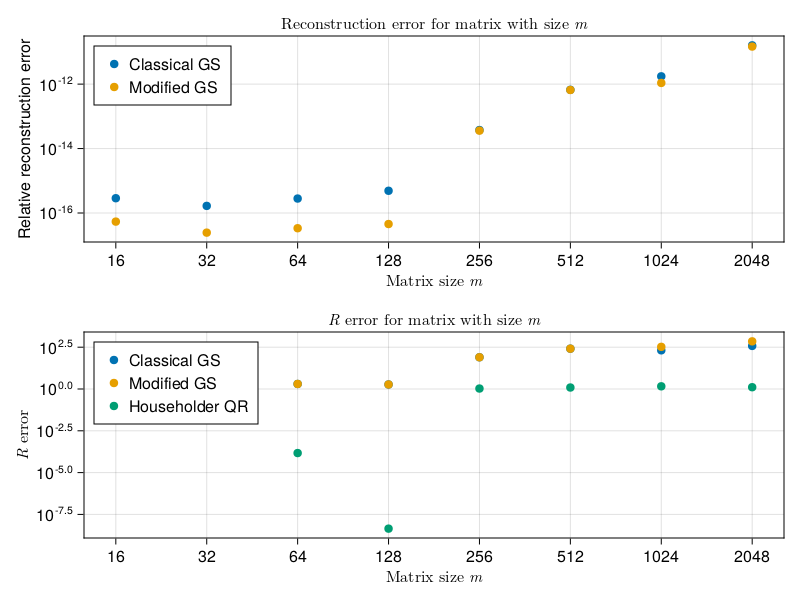
\includegraphics[width=120mm]{HW4_code/error_compare.png}
  \end{center}
  \caption{Relative errors for increasing matrix size and condition number}
  \label{fig:figure1}
\end{figure}

\begin{figure}[htb]
  \begin{center}
  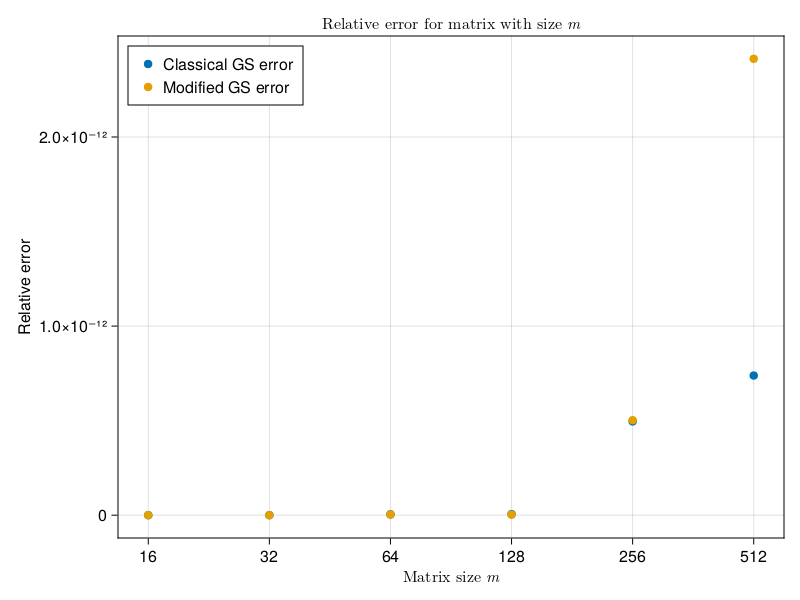
\includegraphics[width=120mm]{HW4_code/error_compare_1.png}
  \end{center}
  \caption{Relative errors for increasing matrix size and condition number}
  \label{fig:figure2}
\end{figure}

\end{document}
